\section{Architectural Overview: Basic TC System}

The \tcs system includes three main components: The \tcontract, the \encname, and the \medname.

The \tcontract (denoted more concisely by \tcont) is a smart contract that acts as the blockchain front-end of the \tc service, and thus an interface between relying contracts and \tc. It accepts datagram requests from requesters and returns corresponding datagrams from \tc. Additionally, the \tcontract manages \tc monetary resources, both fees and gas (in Ethereum). 

The \encname and \medname reside on the \tc server. The \encname runs in an enclave, an SGX-protected execution environment in the server. As enclaves lack network access, the \medname handles bidirectional network traffic on behalf of the \encname, providing network connectivity to the blockchain (the Ethereum system) and to data sources queried by \encname. Additionally, \medname acts as a web server handling off-chain service requests from clients. The \medname is an ordinary user-space application. It does not benefit from special hardware protection and thus, unlike the \encname, can be subverted by an adversarial OS on the \tc server, causing network delays or failures.

The \encname ingests and fulfills datagram requests. To obtain the data composing datagrams, it queries external data sources, specifically HTTPS-enabled internet services. To obtain and keep track of the state of datagram requests, it monitors the state of \tcontract on the blockchain (via scraping). Thus \tcontract forwards datagram requests implicitly to the \tc server. (In the initial version of \tcontract, the \encname's view of the blockchain also comes from a data source.) 

Briefly, then, the end-to-end processing of a datagram request is initiated by a requester \reqcont. \reqcont sends a datagram request to \tcont on the blockchain. Using network services provided by the \medname, the \encname obtains the request from the blockchain. It contacts a data source to obtain the requested data and composes a datagram, which it sends back to \reqcont. Figure~\ref{fig:overview} shows a basic schematic of the \tc system.

As a simple example, \reqcont might request a stock ticker value (e.g., the price of IBM at 3 p.m. on 15 Jan 2016). The \encname would fetch the requested data from an online service (e.g., https://www.google.com/finance) and place it in a datagram for transmission via \tcont to \reqcont.

In addition to servicing datagram requests, the \encname may be queried by a client to provide an off-chain, hardware-backed attestation $\att$ on the state of the \encname---both its executing code and its clock. It is to support this service that \medname includes a web server. We do not depict this service in Figure~\ref{fig:overview}, and defer its discussion to later in the paper.

\vspace{-2mm}
\begin{figure}[h!]
\centering
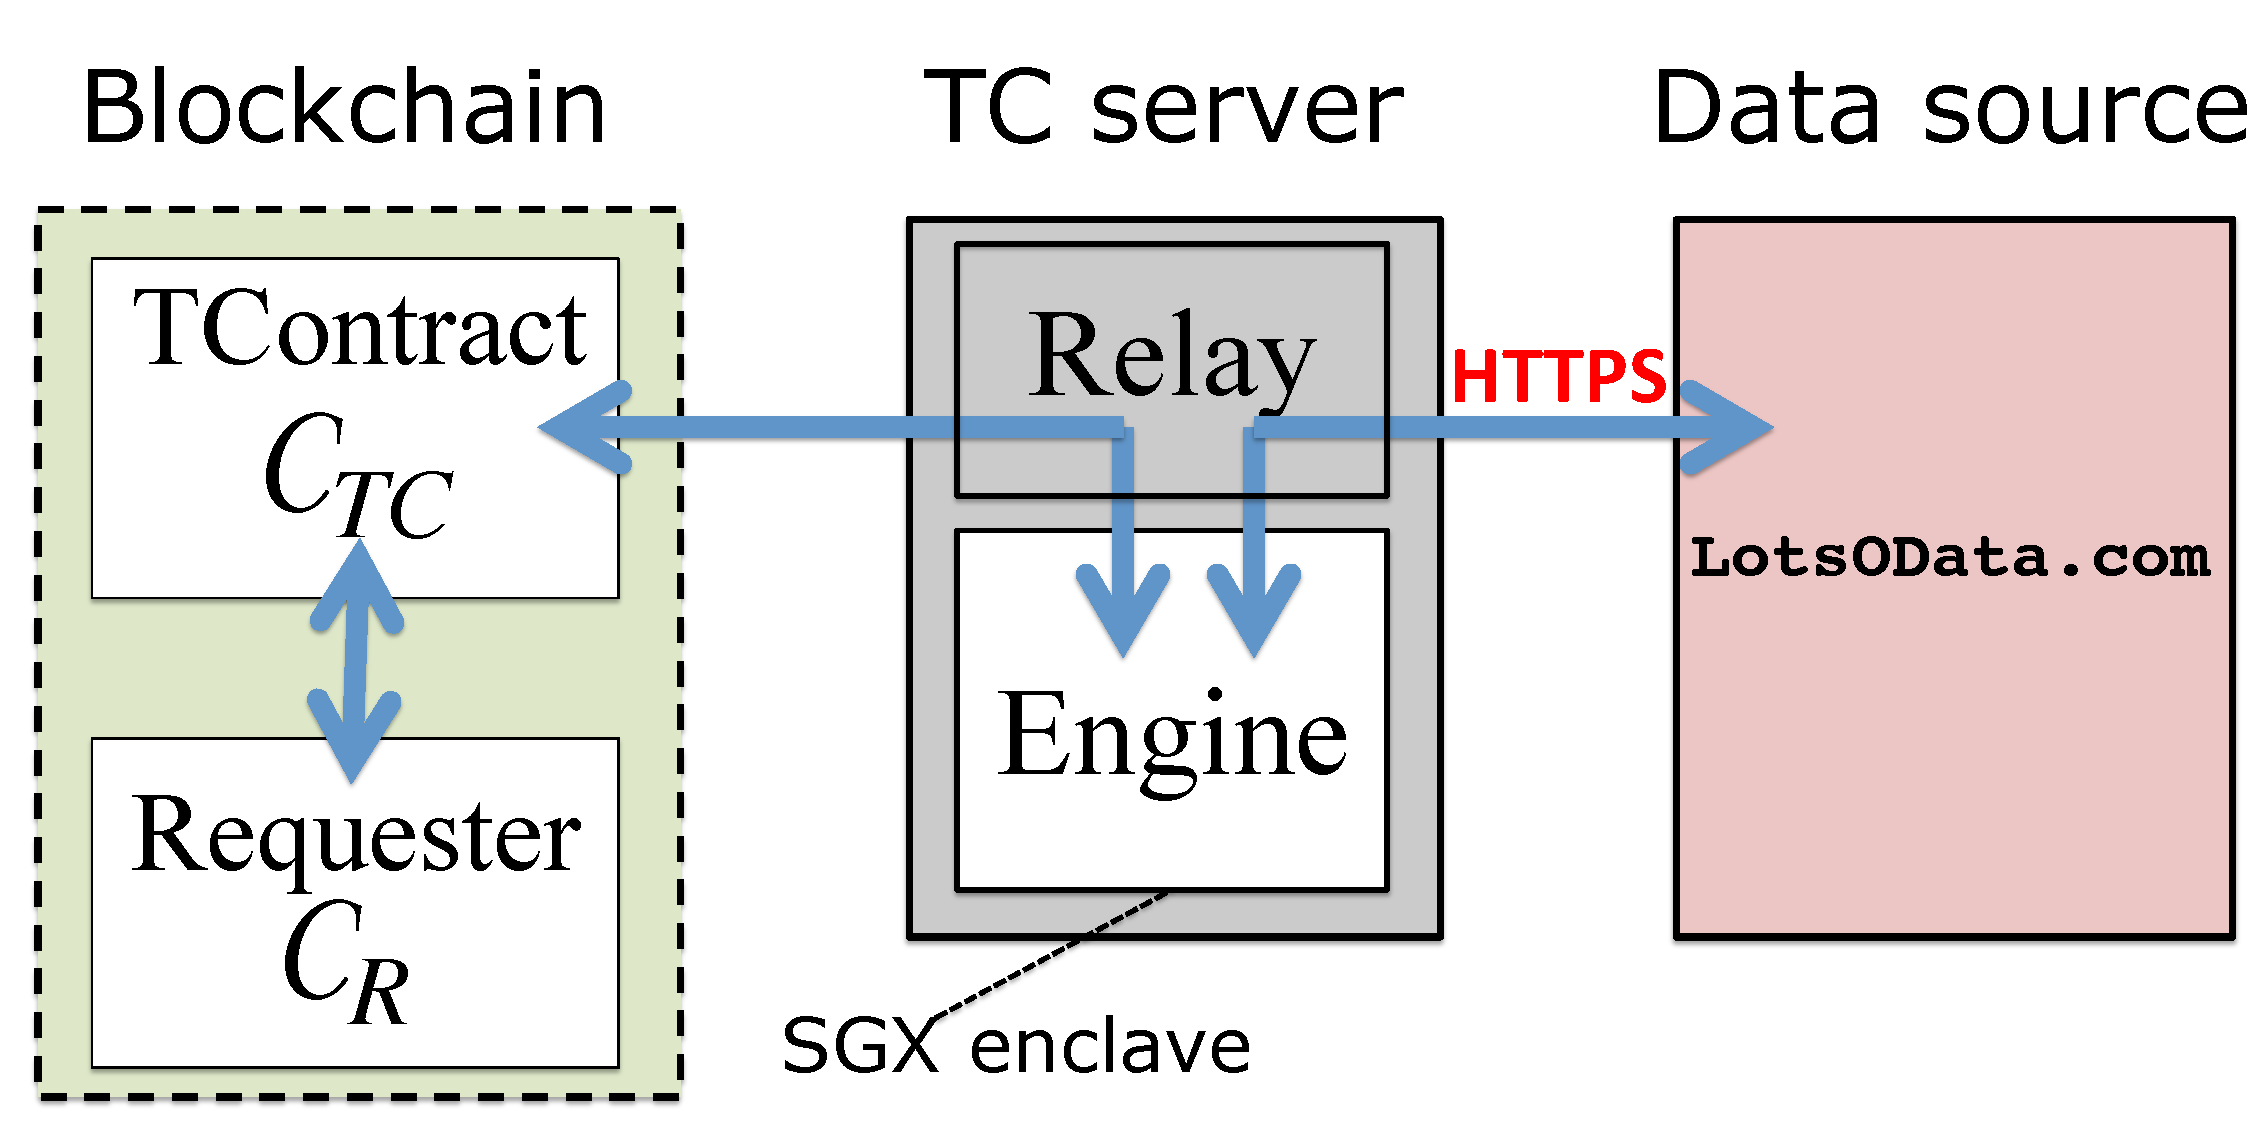
\includegraphics[width=\columnwidth]{OverviewFig}
\caption{{\bf Basic Town Crier architecture.}}
\label{fig:overview}
\end{figure}
\vspace{-2mm}



\subsection{Security model}

Here we given an overview of our security model for \tc, providing more details in our security analysis in section~\ref{}. We assume the following:

\begin{itemize}
\item {\em \encname security:} Leveraging the basic properties of SGX, an attestation $\att$ proves to a verifier (client) about an \encname instance that: (1) The instance is executing correct code, i.e., behaves honestly; (2) For a public key $\pkTC$ included in the attestation, the corresponding private key $\skTC$ is known only to the instance; and (3) The SGX / enclave clock is set to absolute (wall-clock) time $T$ asserted in $\att$, where $T$ is verifiable by a client (requesting a fresh attestation) to within accuracy $\Delta$ (e.g., 100ms).

\item {\em Network communication:} The \medname (and other untrusted components of the \tc server) can tamper with or delay communications to and from the \encname, but cannot otherwise observe or alter the behavior of the \encname. Thus the \medname is simply subsumed by an adversary that controls the network. 

\item {\em Blockchain communication:} Message sources are authenticable, i.e., the originating blockchain address of a message can be correctly identified, and messages are integrity protected, but not confidential. This includes messages sent from the \encname, whose public key $\pkTC$ is bound in \tc to a blockchain account. 
\end{itemize}

\subsection{Design rationale: Role of \tcont}

It is perhaps not immediately evident why our architecture makes use of the contract \tcont to intermediate between \reqcont and the \encname. In principle the \tc service could scrape the blockchain, identify contracts with state explicitly indicating a request for datagrams and send them datagrams and accompanying attestations directly.  This would result in a conceptually simpler protocol, eliminate some in-blockchain message passing, and also ensure that \reqcont consumes only fresh SGX attestations. In contrast, in our design, it is most practical for users to verify an SGX attestation offline at the time \reqcont is created, raising the risk that the attestation goes stale. (Of course, revocation must be handled in either case.)

The rationale for this design choice is twofold: First, \tcont manages the payment of fees (ether and gas) for the \tc service, creating a fair exchange of datagrams for fees. Second, although \reqcont could in principle verify a TC attestation directly, in practice, this would not be practical today. In Ethereum, opcodes for in-contract cryptographic operations are very limited and do not currently support public-key cryptography. (Digital signatures are supported only for messages from non-contract accounts.) 



\subsection{Data flow and notation}

We denote a datagram instance, namely the set of message values associated with a datagram request, by $\dg$. Due to the idiosyncracies of Ethereum and the use of digital signatures for message authentication, the full cycle of datagram processing involves a number of messages. 

A datagram request by \reqcont takes the form of a message $\dgreq$ to \tcont on the blockchain. This message $\dgreq$ includes both a specification $\dgform$ of the requested datagram (e.g., a stock ticker and desired time) and a payment $\dgpay$, which includes (in Ethereum) gas to cover the cost of the request as well as a fee. \tcont receives a return message $\dgret$ from the $\tc$ service. On receiving $\dgret$, \tcont returns the data $\dgm$ it contains (e.g., the desired stock ticker value) to \reqcont. 

We use $\dgi$ to indicate a unique index for a datagram instance. Messages from wallet addresses are authenticated via digital signatures. We use $(\skTC, \pkTC)$ to denote the private / public key pair associated with \tcadd. The key $\skTC$ is stored inside the \encname. (For simplicity, we assume an ability to send signed messages directly to \tcont. Later we explain how Ethereum requires a slightly different approach.)



\subsection{Client API}
\subsection{TC server}
\subsubsection{Trusted executable}
\subsubsection{Untrusted executable}
\subsection{TC Blockchain resources}
These include the TC contract and the addresses from which it sends messages and manages its wallet

There are two parts to the Town Crier blockchain resources:
\begin{itemize}
  \item $\Psgx$ -- An Ethereum wallet whose private key is generated and controlled by the SGX enclave.
  
  \item $\Ctc$ -- An Ethereum contract with two entry points, described in Table~\ref{tbl:tc-contract}.
\end{itemize}
The Town Crier server is responsible for identifying calls to $\Ctc$'s Request request method by scraping the contract activity on the blockchain.
It then replies to those requests through Deliver once it has acquired the necessary data and packaged it into a response.

\begin{table}
\begin{tabularx}{\linewidth}{|@{\hspace{3pt}}r@{\hspace{1ex}}X@{\hspace{3pt}}|}
  \hline

  \multicolumn{2}{|c|}{The Town Crier contract $\Ctc$} \\ [1ex]
  {\bf Request:} & Upon receiving $({\sf type}, {\sf callback}, \${\sf fee})$ from a user $\mathcal{P}$: \\
                 & If $(\${\sf fee} < F_{\rm min}$ or $\${\sf fee} > F_{\rm max})$ \\
                 & \hspace*{1em} Return $\${\sf fee}$ to $\mathcal{P}$ \\
                 & Otherwise do nothing. \\
  {\bf Deliver:} & Upon receiving $({\sf callback}, {\sf data}, \${\sf fee})$ from a user $\mathcal{P}$: \\
                 & If $\mathcal{P} \neq \Psgx$ \\
                 & \hspace*{1em} Return with no effect. \\
                 & Call ${\sf callback}({\sf data})$ providing $\${\sf fee} - F_{\rm min}$ ether as the maximum gas. \\
                 & Send $\${\sf fee}$ ether to $\Psgx$. \\

  \hline
\end{tabularx}
\caption{Definition of the Town Crier contract $\Ctc$.
  Here the minimum fee, $F_{\rm min}$, is the amount of ether necessary to cover the gas costs of Deliver not including the execution of ${\sf callback}$
  and the maximum fee, $F_{\rm max}$, is the maximum amount of ether Town Crier can send as gas to a single execution of Deliver.}
\label{tbl:tc-contract}
\end{table}

\section{Security Model}

Here we assume an adversary which is active on the blockchain, the network, and within the untrusted executable running on the Town Crier server.
However, we assume that the adversary will not execute an arbitrary denial of service attack, but will rather delay messages indefinitely and deliver bogus data whenever such data will be accepted as valid.
Because operations on the blockchain are verifiable and the SGX enclave can attest to what it is running, we assume those are honest.

In this model we show that, for every request which provides a sufficient fee,
a valid authenticated datagram will be delivered to the requested callback location in finite time.
If the request includes an insufficient fee (but is otherwise valid),
the datagram will not be delivered, but the (too-small) fee will still be collected.

\begin{lemma} \label{lem:non-bankrupt-p_sgx}
If seeded with at least $F_{\rm max}$ ether, the $\Psgx$ wallet will have
at least as much money after each transaction as it had before that transaction.
\end{lemma}

\begin{proof}
\ethan{This is actually a proof sketch, I just put it in a proof tag.}

Because all blockchain transactions from $\Psgx$ must be initiated by the SGX enclave and the SGX only calls $\Ctc.{\rm Deliver}$,
we need only reason about what happens inside that function.
Because transactions including $\Ctc$ are transmitted securely into the SGX enclave, it will only see valid requests (ones for which $F_{\rm min} \leq \${\sf fee} \leq F_{\rm max}$) and the arguments it sees for those requests will be correct.
Moreover, it saves the transaction ID of each request it fulfills and never fulfills a request with the same transaction ID twice.
This means that whenever deliver is called, it will be called in connection with a valid request that has not already been delivered.
Thus it suffices to show that:
\begin{enumerate}
  \item The first time a valid request is delivered, $\Ctc$ will contain at least $\${\sf fee}$ ether.
  \item $\${\sf fee}$ is never lower than the amount $\Psgx$ must spend in gas.
  \item The execution of Deliver will never run out of gas (and thus always succeed).
\end{enumerate}

To prove claim 1 we first note that ether can only be removed from $\Ctc$ as part of a call to Deliver from $\Psgx$.
Because $\Psgx$ is honest, it will only make this call in connection with a valid request, and the specified value of $\${\sf fee}$ will always be the fee submitted with that request.
Because $\Ctc$ pays out the specified $\${\sf fee}$ on the call to Deliver, the ether is always exactly the ether stored from a previous, valid, undelivered request, and thus will always be present in $\Ctc$.

To prove claim 2 first note that a request is only considered valid if $\${\sf fee} \geq F_{\rm min}$.
$F_{\rm min}$ is defined so that it is high enough to cover gas costs for all of Deliver except the execution of the provided ${\sf callback}$.
However, ${\sf callback}$ is only given $\${\sf fee} - F_{\rm min}$ ether worth of gas to execute.
Therefore it is impossible for the entire call of Deliver to spend more than $F_{\rm min} + (\${\sf fee} - F_{\rm min}) = \${\sf fee}$ ether on gas.

To prove claim 3 we note that $\${\sf fee} \leq F_{\rm max}$ and, by construction, $\Psgx$ will always provide at least $F_{\rm max}$ in gas for the execution of Deliver.
Therefore we have that $\Psgx$ will always provide at least $\${\sf fee}$ in gas to execute Deliver.
By the argument above, Deliver can never use more than $\${\sf fee}$ in gas, so therefore an SGX-initialized call to Deliver will never run out of gas.
\end{proof}



\begin{lemma} \label{lem:authentic-delivery}
Any data given as an argument to ${\sf callback}$ in $\Ctc$'s Deliver method is verifiably authentic.
\end{lemma}


